% !TeX spellcheck = es_ES
\documentclass[12pt, titlepage]{article}
\usepackage[utf8]{inputenc}
\usepackage[spanish]{babel}
\usepackage{float}
\usepackage[letterpaper, margin=2.5cm]{geometry}
\usepackage[nottoc,notlot,notlof]{tocbibind} % Hace que se agregen las referencias al indice
\usepackage{url}
\usepackage{graphicx} 
\usepackage{listings}
\usepackage{color}
\definecolor{dkgreen}{rgb}{0,0.6,0}
\definecolor{gray}{rgb}{0.5,0.5,0.5}
\definecolor{mauve}{RGB}{253,151,31}

\lstset{frame=tb,
    language=Sql,
    aboveskip=3mm,
    belowskip=3mm,
    showstringspaces=false,
    columns=flexible,
    basicstyle={\small\ttfamily},
    numbers=none,
    numberstyle=\tiny\color{gray},
    keywordstyle=\color{blue},
    commentstyle=\color{dkgreen},
    stringstyle=\color{mauve},
    breaklines=true,
    breakatwhitespace=true,
    tabsize=2,
    morekeywords={use}
}

\title{Tarea 1: Modelo E-R extendido}
\author{Carlos Tonatihu Barrera Pérez \\ Profesor: Hernández Contreras Euler \\ Bases de Datos \\ Grupo: 2CM1 }
\date{12 de marzo de 2017}

\begin{document}
    \maketitle
    \tableofcontents
    \newpage
    \section{Introducción}
    En el diseño de bases de datos existe el modelo entidad-relación que representa la estructura lógica global de la base de datos mediante el uso de conceptos básicos como las entidades, las relaciones y los atributos, estos conceptos y sus derivados nos brindan una gran ayuda en el diseño de la base de datos.\cite{LIBRO}
    \begin{figure}[H]
        \begin{center}
            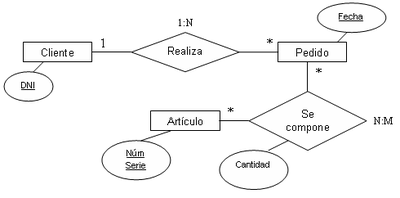
\includegraphics[width=12cm, height=5cm]{img/er.png}
            \caption{Ejemplo de un diagrama entidad-relación}
            \label{fig:modeloER}
        \end{center}
    \end{figure}
    A pesar de que el modelo Entidad-Relación nos permite modelar la mayoría de las características de las bases de datos existen casos en que este modelo no es suficiente por lo que se tiene que utilizar una versión extendida de este llamado modelo E-R extendido.
     \begin{figure}[H]
        \begin{center}
            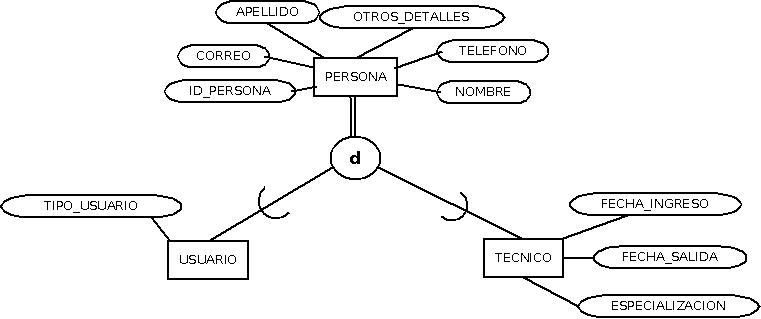
\includegraphics[width=13cm, height=5cm]{img/ere.jpg}
            \caption{Ejemplo de un diagrama entidad-relación extendido}
            \label{fig:modeloERE}
        \end{center}
    \end{figure}
    Este modelo sera explicado en la parte de desarrollo donde se utilizan ejemplos para ilustrar sus principales características ademas de que se presentan los elementos que conforman su notación y algunas herramientas case para poder diseñarlos.
    \section{Desarrollo}
    El modelo entidad-relación extendido (ERE o EER por sus siglas en ingles) es un modelo de datos conceptual capaz de describir la estructura (y funcionalidad) de bases de datos de una forma fácil y directa de entender mediante una notación gráfica.\cite{WEB}
    Además, el modelo ERE incluye todos los conceptos del entidad-relación e incorpora nuevos conceptos los cuales son: \textbf{subclases/superclase}, \textbf{especialización/generalización},\textbf{ herencia} y \textbf{categorías}.
    \subsection{Subclases/Superclases}
    Esta característica se presenta cuando las entidades de los modelos tienen subgrupos de entidades que deben ser representados en el modelo debido a su importancia.\cite{LIBRO1}
    Un ejemplo que ilustra esto se encuentra en la \textit{figura \ref{fig:ejemplo1}} en donde vehículo es la superclase (o entidad de nivel superior) y coche y camión son las subclases (o entidades de nivel inferior).
    \begin{figure}[H]
        \begin{center}
            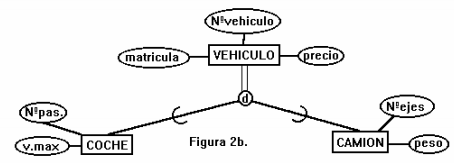
\includegraphics[width=8cm, height=4cm]{img/ejemplo1.png}
            \caption{Un vehículo debe de ser forzosamente un coche o un camión pero no ambos.}
            \label{fig:ejemplo1}
        \end{center}
    \end{figure}
    Es importante mencionar que una entidad no solo puede ser miembro de una subclase sino que también debe de ser miembro de la superclase. Además, una entidad pude ser miembro de varias subclases.
    \subsection{Especialización/Generalización}
    Especialización es el proceso de definir un conjunto de subclases de una superclase. El conjunto se subclases esta basado en algunas características distintivas de las entidades en la superclase.
    
    La generalización es el proceso reverso a la especialización Varias clases con características en común son generalizadas en una superclase.\cite{LIBRO1}
    
    Tanto la especificación como la generalización presentan las siguientes restricciones.
    \begin{itemize}
        \item Definidas por predicado (predicate-defined) o por condición (condition-defined). Usada cuando podemos determinar aquellas entidades que se convertirán en miembros de cada subclase mediante una condición.
        \item Definidas por atributo (attribute-defined). 
        \item Definidas por atributo. Si todas las subclases en una especialización tienen una condición de pertenencia en el mismo atributo de la superclase.
        \item Definida por el usuario (user-defined). Si no existe condición para determinar la pertenencia a una subclase. Ademas la clasificación se hará manualmente.
        \item Restricción de disyunción (disjointness constraint). Puede ser de dos tipos.
            \begin{itemize}
                \item Disjunta (disjoint). La entidad puede ser miembro de una única subclase de la especialización.
                \item Solapada (operlapping). Una misma entidad puede ser miembro de una o mas subclases de una especialización 
            \end{itemize}
        \item Restricción de completitud (completeness constraint). Existen dos tipos.
        \begin{itemize}
            \item Total especifica que cada entidad en la superclase debe ser miembro de alguna subclase.
            \item Parcial permite a las entidades no pertenecer a ninguna subclase.
        \end{itemize}
    \end{itemize}
    \begin{figure}[H]
        \begin{center}
            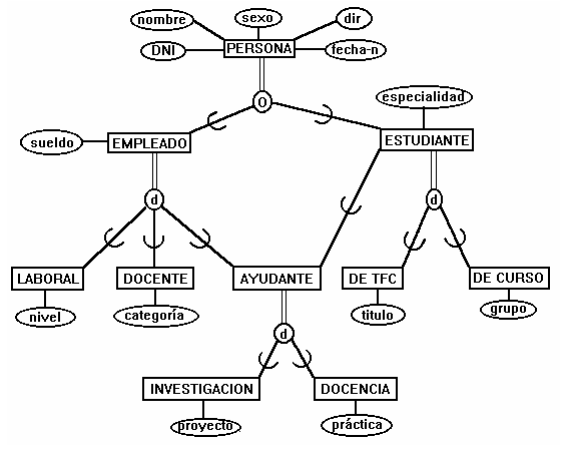
\includegraphics[width=15cm, height=12cm]{img/ejemplo.png}
            \caption{Ejemplo con la mayoría de los elementos de la generalización y la especialización}
            \label{fig:ejemplo}
        \end{center}
    \end{figure}
    \subsection{Herencia}
    Una propiedad de las subclases y superclases creadas mediante la especialización y la generalización es la herencia de atributos. Esto hace referencia a que los atributos de las entidades de nivel superior son heredados por las entidades de nivel inferior esto no ocurre en sentido inverso.\cite{WEB}
    \begin{figure}[H]
        \begin{center}
            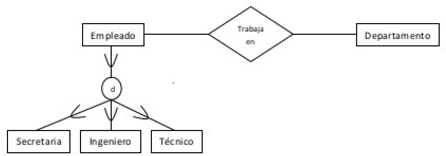
\includegraphics[width=10cm, height=4cm]{img/herencia1.png}
            \caption{Ejemplo de herencia simple.}
            \label{fig:ejemplo2}
        \end{center}
    \end{figure}
    También las subclases heredan la participación en los conjuntos de relaciones en los que participa su superclase. Además la herencia se divide en simple y múltiple en donde la múltiple hace referencia a que una subclase compartida puede tener varias superclases como se presenta en la \textit{figura \ref{fig:ejemplo2}} en este caso se dice que se tiene un retículo, malla o red (lattice), en la herencia simple una subclase tiene solo una superclase un ejemplo de esto se puede observar en la \textit{figura \ref{fig:ejemplo3}} y es básicamente una estructura de árbol.\cite{LIBRO1}
    \begin{figure}[H]
        \begin{center}
            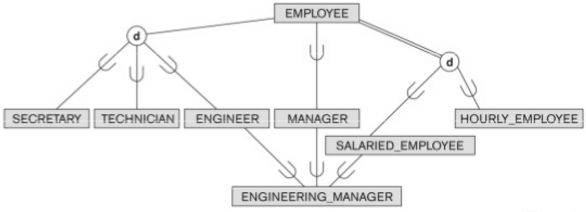
\includegraphics[width=12cm, height=5cm]{img/herencia2.png}
            \caption{En este caso engineering\_manager tiene herencia multiple de engineer, manager y salaried\_employee.}
            \label{fig:ejemplo3}
        \end{center}
    \end{figure}
    \subsection{Categorías}
    Un tipo de unión o categoría es una subclase que representa una colección de objetos que son un subconjunto de la unión de distintos tipos de entidad, las categorías tienen las siguientes características.\cite{LIBRO}
    \begin{itemize}
        \item Siempre tienen dos o mas superclases.
        \item Parcial permite a las entidades no pertenecer a ninguna subclase.
        \item Participación en una categoría Existen dos tipos.
        \begin{itemize}
            \item Total. Si todas las superclases de la categoría deben ser miembros de la categoría Esto también puede modelarse como una generalización disjunta.
            \item Parcial. Si no todas las superclases deben ser miembros de una categoría
        \end{itemize}
    \end{itemize}
    \subsection{Notación y herramientas CASE}
    Los diagramas ERE heredan los elementos que conforman el diseño de los diagramas ER pero agregan nuevos componentes para representar sus características de herencia, superclases/subclases, especialización/generalización y tipo de unión.
    
    Existen varias formas de representar los elementos de este tipo de diagramas pero una muy utilizada es la siguiente.
    En la relación entre superclases y subclases se utiliza el símbolo de pertenencia en la linea.
    \begin{figure}[H]
        \begin{center}
            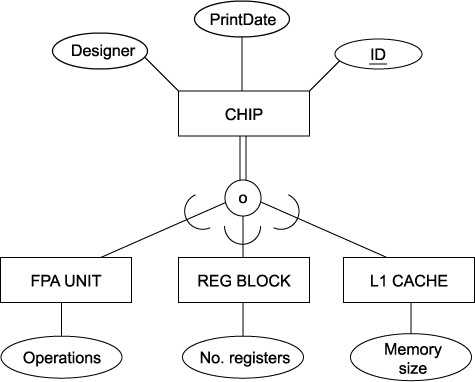
\includegraphics[width=12cm, height=5cm]{img/notacion1.jpg}
            \caption{Ejemplo de herencia simple.}
            \label{fig:notacion1}
        \end{center}
    \end{figure}
    \begin{figure}[H]
        \begin{center}
            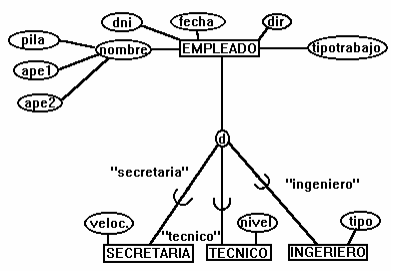
\includegraphics[width=12cm, height=6cm]{img/notacion2.png}
            \caption{Ejemplo de herencia simple.}
            \label{fig:notacion2}
        \end{center}
    \end{figure}
    \begin{figure}[H]
        \begin{center}
            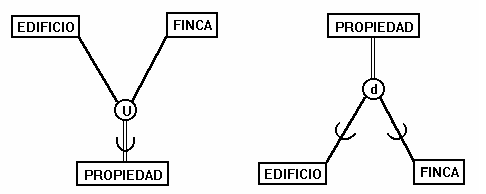
\includegraphics[width=10cm, height=4cm]{img/notacion4.png}
            \caption{Ejemplo de herencia simple.}
            \label{fig:ejemplo4}
        \end{center}
    \end{figure}
    \begin{figure}[H]
        \begin{center}
            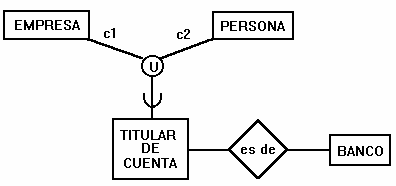
\includegraphics[width=10cm, height=4cm]{img/notacion5.png}
            \caption{Ejemplo de herencia simple.}
            \label{fig:ejemplo5}
        \end{center}
    \end{figure}
    
    Para el desarrollo de este tipo de diagramas existen herramientas CASE que tienen la opción de utilizar elementos de este tipo de diagramas o en su defecto se utilizan diagramas de clases para representar este modelo. Algunas de estas herramientas son.
    \begin{itemize}
        \item Umbrello
        \item StarUML
        \item EERCASE
        \item DB Designer
    \end{itemize}
    \section{Conclusión}
    Los diagramas entidad-relación extendidos son mucho mucho mas completos que los ER por lo que nos ofrecen mas herramientas para del diseño de nuestra base de datos pero debido a su complejidad hay que conocerlos a fondo y los elementos que los conforman para poder utilizarlos de la manera más optima posible ya que de lo contrario en vez de generar un beneficio pueden llegar a ser prejudiciales en el desarrollo de un proyecto. 
    
    Otro punto importante a considerar es en que momento utilizarlo debido a que por su nivel de complejidad es bueno para proyectos que demanden mayor detalle así que en sistemas que necesiten una base de datos pequeña no tan compleja seria una mejor idea utilizar el modelo entidad-relación básico.
    \bibliography{bibliografia} 
    \bibliographystyle{ieeetr}
\end{document}